\documentclass[fleqn, a4paper, 12pt, twoside]{article}
\usepackage{exsheets} %question and solution environments
\usepackage{amsmath, amssymb, amsthm} %standard AMS packages
\usepackage{esint} %integral signs
\usepackage{marginnote} %marginnotes
\usepackage{gensymb} %miscellaneous symbols
\usepackage{commath} %differential symbols
\usepackage{xcolor} %colours
\usepackage{cancel} %cancelling terms
\usepackage[free-standing-units]{siunitx} %formatting units
\usepackage{tikz, pgfplots} %diagrams
	\usetikzlibrary{calc, hobby, patterns, intersections, angles, quotes, spy}
\usepackage{graphicx} %inserting graphics
\usepackage{epstopdf} %converting and inserting eps graphics
\usepackage{hyperref} %hyperlinks
\usepackage{datetime} %date and time
\usepackage{ulem} %underline for \emph{}
\usepackage{xfrac, lmodern} %inline fractions
\usepackage{enumerate, enumitem} %numbered lists
\usepackage{float} %inserting floats
\usepackage[american voltages]{circuitikz} %circuit diagrams
\usepackage{pdflscape} %pages in landscape orientation
\usepackage{setspace} %double spacing
\usepackage{microtype} %micro-typography
\usepackage{listings} %formatting code
	\lstset{language=Matlab}
	\lstdefinestyle{standardMatlab}
	{
		belowcaptionskip=1\baselineskip,
		breaklines=true,
		frame=L,
		xleftmargin=\parindent,
		language=C,
		showstringspaces=false,
		basicstyle=\footnotesize\ttfamily,
		keywordstyle=\bfseries\color{green!40!black},
		commentstyle=\itshape\color{purple!40!black},
		identifierstyle=\color{blue},
		stringstyle=\color{orange},
	}
\usepackage{algpseudocode} %algorithms
\usepackage{algorithm} %algorithms
\usepackage{chronology}
\usepackage{qtree}
\usepackage{varwidth}

\newcommand\numberthis{\addtocounter{equation}{1}\tag{\theequation}} %adds numbers to specific equations in non-numbered list of equations

\theoremstyle{definition}
\newtheorem{example}{Example}
\newtheorem{definition}{Definition}

\theoremstyle{theorem}
\newtheorem{theorem}{Theorem}
\newtheorem{law}{Law}

\newcommand{\curl}{\mathrm{curl\,}}

\newcommand{\divergence}{\mathrm{div\,}}

\makeatletter
\@addtoreset{section}{part} %resets section numbers in new part
\makeatother

\newcommand\blfootnote[1]{%
	\begingroup
	\renewcommand\thefootnote{}\footnote{#1}%
	\addtocounter{footnote}{-1}%
	\endgroup
}

\renewcommand{\marginfont}{\scriptsize \color{blue}}

\renewcommand{\tilde}{\widetilde}

\SetupExSheets{solution/print = true} %prints all solutions by default

%opening
\title{Quantum and Solid State Physics}
\author{Aakash Jog}
\date{2015-16}

\begin{document}

\maketitle
%\setlength{\mathindent}{0pt}

\blfootnote
{	
	\begin{figure}[H]
		
\includegraphics[height = 12pt]{cc.eps}
		\includegraphics[height = 12pt]{by.eps}
		\includegraphics[height = 12pt]{nc.eps}
		\includegraphics[height = 12pt]{sa.eps}
	\end{figure}
	This work is licensed under the Creative Commons Attribution-NonCommercial-ShareAlike 4.0 International License. To view a copy of this license, visit \url{http://creativecommons.org/licenses/by-nc-sa/4.0/}.
} %CC-BY-NC-SA license

\tableofcontents

\newpage
\part{Quantum Physics}

\section{Lecturer Information}

\textbf{Asia Shapira}\\
~\\
E-mail: \href{mailto:asiasapi@gmail.com}{asiasapi@gmail.com}\\

\section{Required Reading}

\begin{enumerate}
	\item Griffiths, D. Introduction to quantum mechanics
\end{enumerate}

\section{Additional Reading}

\begin{enumerate}
	\item Tang: Fundamentals of quantum mechanics, Cambridge press.
	\item Miller, Quantum mechanics for scientists and engineers.
\end{enumerate}

\section{Waves}

\begin{figure}[H]
	\Tree
	[
		.Waves
		[
			.Mechanical
			{
				Need medium for propagation
			}
		]
		[
			.Electromagnetic
			{
				Do not need medium for propagation
			}
		]
	]
\end{figure}

\subsection{1D Wave Equation}

\begin{definition}[1D wave equation]
	The equation
	\begin{align*}
		\dpd[2]{\psi}{t} & = v^2 \dpd[2]{\psi}{x}
	\end{align*}
	where $\psi$ is a function of $x$ and $t$, and $v$ is the velocity of the wave, is called a 1D wave equation.
\end{definition}

\section{Harmonic Waves}

\begin{definition}[Harmonic waves]
	If a wave satisfies the equation
	\begin{align*}
		\psi(x,t) & = A \cos(k x - \omega t + \varphi)
	\end{align*}
	it is called a harmonic wave.\\
	$A$ is called the amplitude of the wave.\\
	$k$ is called the wave number, or spatial frequency of the wave.\\
	$\omega$ is called the angular frequency of the wave.\\
\end{definition}

\begin{definition}[Wavelength]
	For a harmonic wave, a number $\lambda$, such that
	\begin{align*}
		\psi(x) & = \psi(x + \lambda)
	\end{align*}
	is called the wavelength of the wave.
	\begin{figure}[H]
		\begin{tikzpicture}[scale = 0.8]
			\def\xMIN{0};
			\def\xMAX{14};
			\def\yMIN{0};
			\def\yMAX{2};

			\begin{scope}[stealth-stealth, lightgray]
				\draw (\xMIN-1,0) -- (\xMAX+1,0) node [right] {$x$};
				\draw (0,\yMIN-1) -- (0,\yMAX+1) node [above] {$\psi(x)$};
			\end{scope}

			\begin{scope}
				\draw [smooth, domain=\xMIN:\xMAX] plot (\x, {cos(\x r)});
			\end{scope}

			\begin{scope}[|<->|, yshift = -2cm]
				\draw (pi,0) -- (3*pi,0) node [midway, below] {$\lambda$};
			\end{scope}
		\end{tikzpicture}
	\end{figure}
\end{definition}

\begin{definition}[Time period]
	For a harmonic wave, a number $T$, such that
	\begin{align*}
		\psi(t) & = \psi(t + T)
	\end{align*}
	is called the time period of the wave.
	\begin{figure}[H]
		\begin{tikzpicture}[scale = 0.8]
			\def\xMIN{0};
			\def\xMAX{14};
			\def\yMIN{0};
			\def\yMAX{2};

			\begin{scope}[stealth-stealth, lightgray]
				\draw (\xMIN-1,0) -- (\xMAX+1,0) node [right] {$t$};
				\draw (0,\yMIN-1) -- (0,\yMAX+1) node [above] {$\psi(t)$};
			\end{scope}

			\begin{scope}
				\draw [smooth, domain=\xMIN:\xMAX] plot (\x, {cos(\x r)});
			\end{scope}

			\begin{scope}[|<->|, yshift = -2cm]
				\draw (pi,0) -- (3*pi,0) node [midway, below] {$T$};
			\end{scope}
		\end{tikzpicture}
	\end{figure}
\end{definition}

\begin{theorem}
	\begin{align*}
		k & = \frac{2 \pi}{\lambda}
	\end{align*}
	where $k$ is the wave number, and $\lambda$ is the wavelength.
\end{theorem}

\begin{proof}
	If $t = 0$,
	\begin{align*}
		\psi(x) & = A \cos(k x) \\
	\end{align*}
	By the definition of wavelength,
	\begin{align*}
		\psi(x)                & = \psi(x + \lambda)                    \\
		\therefore A \cos(k x) & = A \cos\left( k (x + \lambda) \right) \\
		\therefore k \lambda   & = 2 \pi                                \\
		\therefore k           & = \frac{2 \pi}{\lambda}
	\end{align*}
\end{proof}

\begin{theorem}
	\begin{align*}
		\omega & = \frac{2 \pi}{T}
	\end{align*}
	where $\omega$ is the angular frequency, and $T$ is the time period.
\end{theorem}

\begin{proof}
	If $x = 0$,
	\begin{align*}
		\psi(t) = A \cos(\omega t) \\
	\end{align*}
	By the definition of wavelength,
	\begin{align*}
		\psi(t)                     & = \psi(t + T)                         \\
		\therefore A \cos(\omega t) & = A \cos\left( \omega (t + T) \right) \\
		\therefore \omega T         & = 2 \pi                               \\
		\therefore \omega           & = \frac{2 \pi}{T}
	\end{align*}
\end{proof}

\subsection{Complex Representation of Waves}

Let
\begin{align*}
	\tilde{\psi} & = A e^{i \left( k x - \omega t + \varphi \right)}
\end{align*}
Then,
\begin{align*}
	\psi & = \Re\{\tilde{\psi}\}
\end{align*}

\subsection{Interference of Waves}

\begin{theorem}
	Wave equations are linear, i.e. if $\psi_1$ and $\psi_2$ are solutions to the equation, then $\psi_1 + \psi_2$ is also a solution to the equation.
\end{theorem}

\subsubsection{Interference of Waves with a Phase Difference}

Let
\begin{align*}
	\psi_1 & = A \cos(k x - \omega t + \varphi) \\
	\psi_2 & = A \cos(k x - \omega t)
\end{align*}
Therefore,
\begin{align*}
	\psi_3 & = \psi_1 + \psi_2                                           \\
               & = A \cos(k x - \omega t + \varphi) + A \cos(k x - \omega t) \\
               & = 2 A \cos\left( \frac{\varphi}{2} \right) \cos\left( k x + \omega t + \frac{\varphi}{2} \right)
	\marginnote
	{
		$\because \cos a + \cos b = 2 \cos\left( \frac{a + b}{2} \right) \cos\left( \frac{a - b}{2} \right)$
	}
\end{align*}
Therefore, the resultant wave is a wave with amplitude $2 A \cos\left( \frac{\varphi}{2} \right)$ and phase $\frac{\varphi}{2}$.

\section{Young's Double Slit Experiment (1801)}

This experiment provided substantial proof that light behaves like a wave.

\begin{figure}[H]
	\begin{tikzpicture}
		\def\xMIN{0};
		\def\xMAX{14};
		\def\yMIN{-3};
		\def\yMAX{3};

		\coordinate (S1) at (0,1);
		\coordinate (S2) at (0,-1);

		\draw (0,\yMIN) -- (0,\yMAX);

		\begin{scope}
			\draw ($ (S1) + (-4pt,2pt) $) -- ($ (S1) + (4pt,2pt) $);
			\draw ($ (S1) + (-4pt,-2pt) $) -- ($ (S1) + (4pt,-2pt) $);
			\fill [white] ($ (S1) + (-4pt,-2pt) $) rectangle ($ (S1) + (4pt,2pt) $);
		\end{scope}

		\begin{scope}
			\draw ($ (S2) + (-4pt,2pt) $) -- ($ (S2) + (4pt,2pt) $);
			\draw ($ (S2) + (-4pt,-2pt) $) -- ($ (S2) + (4pt,-2pt) $);
			\fill [white] ($ (S2) + (-4pt,-2pt) $) rectangle ($ (S2) + (4pt,2pt) $);
			\draw ($ (S2) + (6pt,10pt) $) -- ($ (S2) + (6pt,-10pt) $);
		\end{scope}

		\begin{scope}[xshift = 5cm, tension = 100]
			\draw (0,\yMIN) -- (0,\yMAX);
			
			\draw [yshift = 1cm] (0,2) to [out = -90, in = 90] (-0.5,0) to [out = -90, in = 90] (0,-2);
		\end{scope}
	\end{tikzpicture}
	\caption{Intensity of light with only first slit open}
\end{figure}

\begin{figure}[H]
	\begin{tikzpicture}
		\def\xMIN{0};
		\def\xMAX{14};
		\def\yMIN{-3};
		\def\yMAX{3};

		\coordinate (S1) at (0,1);
		\coordinate (S2) at (0,-1);

		\draw (0,\yMIN) -- (0,\yMAX);

		\begin{scope}
			\draw ($ (S1) + (-4pt,2pt) $) -- ($ (S1) + (4pt,2pt) $);
			\draw ($ (S1) + (-4pt,-2pt) $) -- ($ (S1) + (4pt,-2pt) $);
			\fill [white] ($ (S1) + (-4pt,-2pt) $) rectangle ($ (S1) + (4pt,2pt) $);
			\draw ($ (S1) + (6pt,10pt) $) -- ($ (S1) + (6pt,-10pt) $);
		\end{scope}

		\begin{scope}
			\draw ($ (S2) + (-4pt,2pt) $) -- ($ (S2) + (4pt,2pt) $);
			\draw ($ (S2) + (-4pt,-2pt) $) -- ($ (S2) + (4pt,-2pt) $);
			\fill [white] ($ (S2) + (-4pt,-2pt) $) rectangle ($ (S2) + (4pt,2pt) $);
		\end{scope}

		\begin{scope}[xshift = 5cm, tension = 100]
			\draw (0,\yMIN) -- (0,\yMAX);
			
			\draw [yshift = -1cm] (0,2) to [out = -90, in = 90] (-0.5,0) to [out = -90, in = 90] (0,-2);
		\end{scope}
	\end{tikzpicture}
	\caption{Intensity of light with only second slit open}
\end{figure}

\begin{figure}[H]
	\begin{tikzpicture}
		\def\xMIN{0};
		\def\xMAX{14};
		\def\yMIN{-3};
		\def\yMAX{3};

		\coordinate (S1) at (0,1);
		\coordinate (S2) at (0,-1);

		\draw (0,\yMIN) -- (0,\yMAX);

		\begin{scope}
			\draw ($ (S1) + (-4pt,2pt) $) -- ($ (S1) + (4pt,2pt) $);
			\draw ($ (S1) + (-4pt,-2pt) $) -- ($ (S1) + (4pt,-2pt) $);
			\fill [white] ($ (S1) + (-4pt,-2pt) $) rectangle ($ (S1) + (4pt,2pt) $);
		\end{scope}

		\begin{scope}
			\draw ($ (S2) + (-4pt,2pt) $) -- ($ (S2) + (4pt,2pt) $);
			\draw ($ (S2) + (-4pt,-2pt) $) -- ($ (S2) + (4pt,-2pt) $);
			\fill [white] ($ (S2) + (-4pt,-2pt) $) rectangle ($ (S2) + (4pt,2pt) $);
		\end{scope}

		\begin{scope}[xshift = 5cm, tension = 100]
			\draw (0,\yMIN) -- (0,\yMAX);
			
			\draw (0,2.5) to [out = -90, in = 90] (-0.3,2) to [out = -90, in = 90] (0,1.5);
			\draw (0,1.5) to [out = -90, in = 90] (-0.6,1) to [out = -90, in = 90] (0,0.5);
			\draw (0,0.5) to [out = -90, in = 90] (-0.9,0) to [out = -90, in = 90] (0,-0.5);
			\draw (0,-1.5) to [out = 90, in = -90] (-0.6,-1) to [out = 90, in = -90] (0,-0.5);
			\draw (0,-2.5) to [out = 90, in = -90] (-0.3,-2) to [out = 90, in = -90] (0,-1.5);
		\end{scope}
	\end{tikzpicture}
	\caption{Intensity of light with both slits open}
\end{figure}

\subsection{YDSE with Classical Particles}

If the double slit experiment is performed with classical particles, instead of waves, the intensities add up.
There is no fringe pattern, as observed in the experiment with waves.

\section{The Photoelectric Effect}

The first experiment in which the photoelectric effect was observed was performed by Hertz in 1887.\\
Two metallic plates, acting as electrodes were arranged as shown.
They were connected to a voltage source $\Delta V$, as shown.
\begin{figure}[H]
	\begin{tikzpicture}
		\draw (1,0) rectangle (2,2);
		\draw (-1,0) rectangle (-2,2);

		\draw (1.5,0) -- (1.5,-1);
		\draw (-1.5,0) -- (-1.5,-1);
		\draw (1.5,-1) to [battery1 = $\Delta V$] (-1.5,-1);

		\begin{scope}[stealth-]
			\foreach \y in {0.5,1,1.5}
			{
				\draw (2,\y) -- ++(1,0);
			}
		\end{scope}

		\node [right] at (3,1) {light};

		\draw [-stealth] (0.75,1) -- (-0.75,1) node [midway, above] {$e^-$};
	\end{tikzpicture}
\end{figure}
The results observed were as shown.\\
\begin{enumerate}[leftmargin=*]
	\item
		The relationship between $\Delta V$ and the current in the wire was observed to be as shown.
		\begin{figure}[H]
			\begin{tikzpicture}
				\def\xMIN{-3};
				\def\xMAX{8};
				\def\yMIN{0};
				\def\yMAX{2};
		
				\begin{scope}[stealth-stealth, lightgray]
					\draw (\xMIN-1,0) -- (\xMAX+1,0) node [right] {$\Delta V$};
					\draw (0,\yMIN-1) -- (0,\yMAX+1) node [above] {$I$};
				\end{scope}
		
				\begin{scope}
					\draw (\xMIN,0) -- (0,1) -- (\xMAX,1);
					\draw (\xMIN,0) -- (0,2) -- (\xMAX,2);
				\end{scope}
		
				\node [below] at (\xMIN,0) {$\Delta V_s$(stopping voltage)};
			\end{tikzpicture}
		\end{figure}
		The conclusions were as follows.
		\begin{enumerate}
			\item
				If the light intensity is constant, a specific amount of electrons is emitted.
				Therefore, the current is constant, and independent of $\Delta V$.\\
			\item
				If $\Delta V >> 0$, all electrons emitted reached the other plate, and hence contributed to the current.\\
				If $\Delta V < 0$, some electrons were unable to reach the other plate, and hence did not contribute to the current.
			\item
				$\Delta V_s$ is not dependent on the intensity of the light.
		\end{enumerate}
		~\\
		As the energy of an electron is conserved,
		\begin{align*}
			E_{K_i} + E_{P_i} & = E_{K_f} + E_{P_f}
		\end{align*}
		Therefore, if the electron barely reaches the other plate, i.e. if the voltage is $\Delta V_s$
		\begin{align*}
			E_{K_i} + 0             & = (-e) (-\Delta V_s) \\
			\therefore e \Delta V_s & = E_K
		\end{align*}
		Therefore, as $\Delta V_s$ is independent of the intensity of light, the kinetic energy of the emitted electrons is also independent of the intensity of light.\\
	\item
		The relationship between the kinetic energy of the emitted electrons, and the frequency of the incident light was observed to be as shown.
		\begin{figure}[H]
			\begin{tikzpicture}
				\def\xMIN{0};
				\def\xMAX{8};
				\def\yMIN{0};
				\def\yMAX{2};
		
				\begin{scope}[stealth-stealth, lightgray]
					\draw (\xMIN-1,0) -- (\xMAX+1,0) node [right] {$f$};
					\draw (0,\yMIN-1) -- (0,\yMAX+1) node [above] {$E_K$};
				\end{scope}
		
				\begin{scope}
					\draw (1,0) -- ++(2,\yMAX) node [above left] {metal 1};
					\draw [xshift = 1cm] (1,0) -- ++(2,\yMAX) node [above] {metal 2};
					\draw [xshift = 2cm] (1,0) -- ++(2,\yMAX) node [above right] {metal 3};
				\end{scope}
			\end{tikzpicture}
		\end{figure}
		The conclusions were as follows.
		\begin{enumerate}
			\item
				There is a cutoff frequency, i.e. a frequency below which no electrons are emitted.
			\item
				The kinetic energy of the emitted electrons is linearly dependent on the frequency of light.
		\end{enumerate}
\end{enumerate}
~\\
These conclusions were inconsistent with the accepted notion of light being a wave.

\subsection{Einstein's Explanation of the Photoelectric Effect (1905)}

According to Einstein's explanation, light is a stream of particles, called photons.
Each photon has energy equal to $h f$, where $h$ is Planck's constant, and $f$ is the frequency of the light, which is in fact a property of the wave nature of the light.
This theory can explain the conclusions of Hertz's experiment, which could not be explained by classical theories.\\
According to the explanation, each material has a property called the work function ($W$).
The fact that there exists a cutoff voltage is justified due to this energy barrier.
For an electron to be emitted, it needs to be provided energy to overcome this barrier.
The cutoff frequency is such that all energy in a photon of this frequency to be used to overcome the work function.\\
Therefore,
\begin{align*}
	h f_{\textnormal{cutoff}} & = W
\end{align*}
Also, as each photon provides all its energy to a single electron, increasing the intensity of light just increases the number of electrons emitted, but does not increase the kinetic energy of the emitted electrons.

\newpage
\part{Solid State Physics}

\section{Lecturer Information}

\textbf{Tammy Ben-Yaacov}\\
~\\
E-mail: \href{mailto:tammybenyaacov@gmail.com}{tammybenyaacov@gmail.com}\\

\section{Required Reading}

\begin{enumerate}
	\item Streetman, B. Solid State Electronic Devices
\end{enumerate}

\section{Additional Reading}

\begin{enumerate}
	\item Kittel, Introduction to solid state physics, John Wiley \& Sons.
	\item Pierret. Advanced semiconductor Fundamentals, Prentice Hall.
	\item Ashcroft, Solid State Physics, Harcourt college publishers.
\end{enumerate}

\section{Electrons}

\begin{definition}[Particle nature of electrons]
	An electron behaves as a negatively charged charge carrying particle.\\
	The magnitude of the charge on it is
	\begin{align*}
		q & = 1.602 \times 10^{-19} \coulomb
	\end{align*}
	Its mass is
	\begin{align*}
		m_0 & = 9.11 \times 10^{-31} \kilogram
	\end{align*}
\end{definition}

\begin{definition}[Wave nature of electrons]
	Electrons exhibit wave-like properties, in addition to particle-like properties.\\
	The energy transmitted by a wave is
	\begin{align*}
		E & = h \nu \\
                  & = \frac{h c}{\lambda}
	\end{align*}
	where
	\begin{align*}
		h       & = \text{Planck's constant} \left( 6.626 \times 10^{-34} \right) \\
		\nu     & = \text{frequency}                                              \\
		c       & = \text{speed of light}                                         \\
		\lambda & = \text{wavelength}
	\end{align*}
\end{definition}

\section{Semiconductors}

\begin{law}[Ohm's Law]
	The voltage across two points on a conductor is directly proportional to the current through the conductor.
	The constant of proportionality is called the resistance of the conductor.
	\begin{equation*}
		\frac{V}{I} = R
	\end{equation*}
	\label{Ohm's_Law}
\end{law}

\begin{law}[Microscopic Ohm's Law]
	\begin{equation*}
		\overrightarrow{J}  = \sigma \overrightarrow{E}
	\end{equation*}
	where $\overrightarrow{J}$ is the current density, $\sigma$ is the conductivity, $\overrightarrow{E}$ is the electric field in the resistor.
	\label{Microscopic_Ohm's_Law}
\end{law}

\begin{definition}[Resistivity]
	If
	\begin{equation*}
		R = \rho \frac{L}{A}
	\end{equation*}
	where $R$ is the resistance of the resistor, $L$ is the length of the resistor, and $A$ is the cross-sectional area of the resistor, then $\rho$ is called the resistivity of the resistor.\\
	$\sigma = \frac{1}{\rho}$ is called the conductivity of the resistor.\\
	They are constant for a particular material.
\end{definition}

\begin{figure}[H]
	\begin{tikzpicture}
		\begin{scope}
			\draw [green] (0,0) -- (3,0);
			\draw [yellow] (3,0) -- (6,0);
			\draw [-stealth, red] (6,0) -- (9,0);
			\node [right] at (9,0) {$\rho$};
		\end{scope}

		\begin{scope}
			\draw ($ (3,0) + (0,0.1) $) -- ($ (3,0) + (0,-0.1) $) node [below] {$10^{-5}$};

			\draw ($ (6,0) + (0,0.1) $) -- ($ (6,0) + (0,-0.1) $) node [below] {$10^6$};
		\end{scope}

		\begin{scope}
			\node [above] at (1.5,0) {Conductors};
			\node [above] at (4.5,0) {Semiconductors};
			\node [above] at (7.5,0) {Insulators};
		\end{scope}
	\end{tikzpicture}
\end{figure}

\subsection{Control Factors}

The major factors which affect the conductivity of a material are

\begin{enumerate}
	\item Temperature
	\item Chemical composition
		\begin{enumerate}
			\item Atomic bonding
			\item Crystal structure
			\item Charge carriers in the crystal
		\end{enumerate}
	\item Optical effects
	\item Doping
\end{enumerate}

\subsection{Chemical Makeup}

\begin{table}[H]
	\begin{tabular}{c|c|c|c|c}
		$\mathrm{II}$ & $\mathrm{III}$ & $\mathrm{IV}$ & $\mathrm{V}$ & $\mathrm{VI}$ \\
		\hline
                              & B              & C             & N            & O             \\
                              & Al             & Si            & P            & S             \\
		Zn            & Ga             & Ge            & As           &               \\
		Cd            & In             &               &              &               \\
	\end{tabular}
\end{table}

\begin{enumerate}
	\item Easily available, hence economical
	\item Performs better at higher temperatures
	\item Can be converted to silica on heating
\end{enumerate}

\begin{figure}[H]
	\Tree
	[
		.Semiconductors
		[
			.Elemental
		]
		[
			.Compound
			[
				.{Binary Compound SCs}
				[
					.{$\mathrm{III}$-$\mathrm{V}$}
					{
						GaAs, InP, GaN
					}
				]
				[
					.{$\mathrm{II}$-$\mathrm{VI}$}
					{
						ZnO
					}
				]
			]
			[
				.{Ternary Compound SCs}
				{
					AlGaAs, InGaN
				}
			]
		]
	]
	\caption{Classification of Semiconductors}
\end{figure}

\begin{question}
	A sample of Germanium has resistivity $\rho = 0.46 \ohm\metre$.
	The dimensions of the sample are
	\begin{align*}
		l & = 50 \si{\micro\metre}  \\
		h & = 0.2 \si{\micro\metre} \\
		w & = 1 \si{\micro\metre}
	\end{align*}
	Find the resistance of the sample and the conductivity of the material.
\end{question}

\begin{solution}
	\begin{align*}
		\rho & = 0.46 \si{\ohm\metre} \\
                     & = 46 \si{\ohm\centi\metre}
	\end{align*}
	Therefore,
	\begin{align*}
		\sigma & = \frac{1}{\rho}                     \\
                       & = \frac{1}{46 \si{\ohm\centi\metre}} \\
                       & = 0.022 \si{\per \ohm \per \centi\metre}
	\end{align*}
	Therefore,
	\begin{align*}
		l & = 50 \micro\metre \\
                  & = 50 \times 10^{-4} \centi\metre
	\end{align*}
	Therefore,
	\begin{align*}
		R & = \rho \frac{l}{A} \\
                  & = 11500 \times 10^{-4} \ohm
	\end{align*}
\end{solution}

\begin{question}
	A sample of Germanium has resistivity $\sigma$.
	The dimensions of the sample are as shown.
	\begin{figure}[H]
		\begin{tikzpicture}
			\def\C{3};
			\def\L{5};
			\def\B{2};
			\def\W{1};

			\begin{scope}
				\draw (0,0) -- (\L,0) -- (\L,\B) -- (0,\C) -- cycle;
				\draw [xshift = \W cm, yshift = \W cm] (0,0) -- (\L,0) -- (\L,\B) -- (0,\C) -- cycle;

				\draw (0,0) -- ++(\W,\W);
				\draw (\L,0) -- ++(\W,\W);
				\draw (\L,\B) -- ++(\W,\W);
				\draw (0,\C) -- ++(\W,\W);
			\end{scope}

			\begin{scope}[stealth-stealth]
				\draw [xshift = -10] (0,0) -- (0,\C) node [midway, left] {$C$};
				\draw [yshift = -10] (0,0) -- (\L,0) node [midway, below] {$L$};
				\draw [xshift = 10] ($ (\L,0) + (\W,\W) $) -- ($ (\L,\B) + (\W,\W) $) node [midway, right] {$B$};
				\draw [xshift = 10, yshift = -10] (\L,0) -- ++(\W,\W) node [midway, below right] {$W$};
			\end{scope}
		\end{tikzpicture}
	\end{figure}
	Find the relationship between $R$ and $\sigma$.
\end{question}

\begin{solution}
	Consider a slice with height $h$, width $w$, and thickness $\dif x$.
	Therefore, the cross-sectional area of the elemental slice is
	\begin{align*}
		\dif A & = w h                                    \\
                       & = w \left( \frac{B - C}{L} x + C \right) \\
                       & = w \left( \frac{B x - C (L - x)}{L} \right)
	\end{align*}
	Therefore,
	\begin{align*}
		\dif R & = \frac{\dif x}{\sigma w h} \\
                       & = \frac{L \dif x}{\sigma w \left( B x - C (L - x) \right)}
	\end{align*}
\end{solution}

\section{Types of Materials}

Atoms tend to arrange themselves in such a way that the resultant energy is minimized.

\begin{figure}[H]
	\Tree
	[
		.Materials
		[
			.Amorphous
			{
				\begin{varwidth}{4cm}
					No well-defined structure
				\end{varwidth}
			}
		]
		[
			.Polycrystalline
			{
				\begin{varwidth}{4cm}
					Many small regions, each having well organized atomic structure
				\end{varwidth}
			}
		]
		[
			.Crystalline
			{
				\begin{varwidth}{4cm}
					Long range 3D order of atoms, with repeating unit cells, throughout the entire solid
				\end{varwidth}
			}
		]
	]
	\caption{Classification of Materials}
\end{figure}

Semiconductor devices can use all of these types of materials.\\
\begin{figure}[H]
	\begin{tikzpicture}
		\def\h{2};
		\def\l{6};

		\begin{scope}
			\draw (0,0) rectangle ++(\l,\h);

			\node [left] at (0,\h/2) {$S$};

			\node at (\l/2,\h/2) {Si substrate (crystalline)};
		\end{scope}

		\begin{scope}[yshift = \h cm]
			\draw (0,0) rectangle ++(\l,\h);

			\node [left] at (0,\h/2) {$O$};

			\node at (\l/2,\h/2) {SiO$_2$ (amorphous)};
		\end{scope}

		\begin{scope}[yshift = 2*\h cm]
			\draw (0,0) rectangle ++(\l,\h);

			\node [left] at (0,\h/2) {$M$};

			\node at (\l/2,\h/2) {poly Si (polycrystalline)};
		\end{scope}
	\end{tikzpicture}
	\caption{MOS which uses all three types of materials}
\end{figure}

\section{Bohr's Model}

According to Bohr's model of the atom, electrons can have discrete energy levels only.
The electrons in an atom are arranged in the order of filling electronic shells, given by the Aufbau Principle.\\
The energy of a free electron is called $E_{\textnormal{vac}}$.
This is used as a reference energy.

\end{document}
